\section{Continuous phase transitions}

In order to address the behavior of a system during a continuous phase transition we can imagine to work in a situation like the one of an unstable binary material. In that case we have that the system wants to generate areas in two different phases and since it's unstable as it is the process that will go through in forming them is a continuous transformation that naturally generates gradients of concentration inside the material. On a more general level we can say that the concentration is the order parameter $\xi$ inside the material and the transformation is naturally generating a gradient $\grad \xi$ inside the system that we want to study. 
\begin{figure}[b]
    \centering
    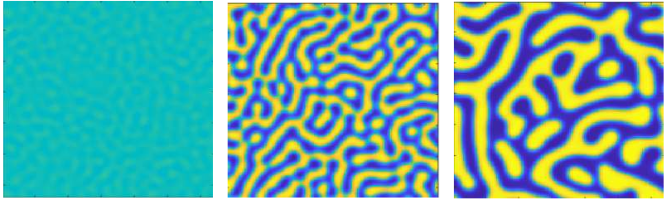
\includegraphics[width=0.8\textwidth]{Immagini/ContPhaseTrans.png}
    \caption{
        Result of a simulation to represent a phase transition in a binary alloy showing in different colors different densities that can be interpreted as the order parameter of the system.
    }
    \label{fig:ContPhaseTrans}
\end{figure}
A great example of this is shown in \figref{fig:ContPhaseTrans}, where the material starts from an ordered situation with uniform density to then naturally create domains generating disorder.

To study such a phenomenon we should not focus our attention only on the domain that are forming inside the material, but an important contribution to the free energy is given by the interfacial regions. The latter are the region of space where the system goes from one domain to another, so the position where $\grad \xi$ is effectively large and non-zero. In fact, such interfaces have a large role in the creation of the new phases since their number is really large in the first part of the transformation driving it at its core. Still, the presence of a gradient needs to generate an increase of $G(\xi)$ due to the fact that the minima of the free energy are represented by the order parameter in the domain, $\xi_\alpha$ and $\xi_\beta$. This means that, for $\xi$ in between those two, present in the wall domain composing the interfaces, necessarily has higher free energy overall increasing it. Therefore, one may ask why they exist and are not reduced to the minimum, and the reason for it can be understood by making the example of magnetic domain in a ferromagnetic material. We know how the gain in energy inside a magnetic domain is due to \textbf{exchange interaction} between spins that prefers to have aligned spin minimizing the energy and increase it otherwise. In this situation having two domains with opposite spins one next to the other highly increase the energy, so that the presence of a gradient that smooth out the interaction is favorable. The question then becomes, how large should such interface be in order for it be effectively be energetically favorable giving rise to the generation of the domains, and how do they evolve? That's the question we are going to answer right now.

\subsection{Cahn-Hilliard equation}

To start modelling the evolution of the system during a phase transition we need to write down a form for the free energy focussing on the local free energy, that we will call $f^{hom}$. We will assume that such a function will depend on the order parameter and it's gradient, allowing us to write down a Taylor expansion of it near the value of $\grad \xi = 0$
\begin{equation}
    f(\xi, \grad\xi) = f^{hom}(\xi) + \pdv{f^{hom}}{\grad \xi}\vdot \grad\xi + \pdv[2] {f^{hom}}{\grad \xi} \grad\xi \vdot \grad \xi.
\end{equation}
We can simplify such a form by noticing that if we change variable $\xi \to -\xi$ also the gradient change sign having that the first order term will modify the energy of the system. That is an absurd since a simple change of variable can't change the physics of the system having that the first derivative respect to the gradient needs to be zero. We can then define $K$ as the second derivative term to end up with the following form
\begin{equation}
    \label{eq:LocalFreeEnerg}
    f(\xi, \grad\xi) = f^{hom}(\xi) + K\grad \xi^2.
\end{equation}
The two terms present behaves so that the first wants to eliminate interfaces since works simply as the local free energy, meaning that has minima for the values of $\xi$ corresponding to the domains and increase as the order changes. Instead, the second term goes against that pushing for the creation of larger interfaces so that $\grad\xi$ is more extended but lower in absolute value along the material. In fact, if no interface would be present the gradient between two domains would have $\abs{\grad\xi} \to \infty$ rising a lot the value of the second term.

Therefore, the \eqref{eq:LocalFreeEnerg} will allow us to model the behavior of the system in general giving us insights on the form of the interfaces. As a matter of facts, it's possible to use such a form to arrive at the following simple result.
\thm{Interface properties}
{
    Inside a continuous phase transformation where the local free energy can be written as in \eqref{eq:LocalFreeEnerg} the width of the domain interfaces and the surface free energy are given by
    \begin{align}
        &\delta = \sqrt{\frac{K}{\mean{f^{hom}}}}, &\gamma = 2\sqrt{K\mean{f^{hom}}}.
    \end{align}
}
\pf{Proof}
{
    We can write down the total energy in the proximity of an interface by integrating the local free energy so that
    \begin{equation}
        \label{eq:TotalFreeEnergyInter}
        F = \int_V \left[ f^{hom}(\xi) + K\left( \dv{\xi}{x} \right)^2 \right]\dd V,
    \end{equation}
    where we assumed that the interface is only in direction $x$ so that the gradient is present only in that component. We can then average the quantity over the volume of the interface by multipling and dividing for $A\delta$, where $A$ is the area of the interface and $\delta$ the width
    \begin{equation}
        F = A\delta\left[ \mean{f^{hom}} + K \mean{\left( \dv{\xi}{x} \right)^2} \right].
    \end{equation}
    The width of the interface can then be set to $\delta \approx \dd x/\dd\xi$ having that the final form of the energy is
    \begin{equation}
        F \approx A\left[ \mean{f^{hom}}\delta + \frac{K}{\delta} \right].
    \end{equation}
    By minimizing this value one can find the wanted value of the width that minimize the free energy and then by substitute it inside $F$ and dividing it by $A$ also $\gamma$ can be computed.
}
\noindent
This is the result we expected after the previous description of the energy. In fact, we can see that as the parameter $K$, related to the gradient term, increase the width of the interfaces inside the material, while the average value of $f^{hom}$ decrease them, exactly as we said before.

Know that we know how the interfaces and the free energy look like we can focus on the dynamics of the system. In particular, is possible by working on the total free energy of the system to define a particular quantity that help us to study the evolution of a general order parameter.
\thm{Generalized diffusion potential}
{
    Inside a continuous phase transformation where the local free energy can be written as in \eqref{eq:LocalFreeEnerg} a generalized chemical potential can be defined describing the local evolution of the order parameter
    \begin{equation}
        \Phi(\vb{r}) = \pdv{f^{hom}}{\xi} - 2K\laplacian \xi.
    \end{equation}
}
\pf{Proof}
{
    We can write down the total free energy of the system as in \eqref{eq:TotalFreeEnergyInter} and then try to minimize it by taking its functional derivative. Therefore, we can set $\xi \to \xi + \dd \xi$ to find out the following form for the variation
    \begin{equation}
        \delta F = \int_V \left[ \pdv{f^{hom}}{\xi}\delta\xi + 2K\grad\xi\vdot \grad(\delta\xi) \right],
    \end{equation}
    then we can use the vector identity $\grad\xi\vdot \grad(\delta\xi) = \grad\vdot(\delta\xi\grad\xi) - \delta\xi\laplacian\xi$ alongside Gauss theorem to have
    \begin{equation}
        \delta F  = \int_V\left[ \pdv{f^{hom}}{\xi} - 2K\laplacian \xi\right]\delta \xi\dd V - \int_{\partial V} \delta\xi\grad\xi\vdot \dd \vb{A}.
    \end{equation}
    The integral over the area gives no contribution in the thermodynamic limit since the volume to area ratio becomes so large that the volume part is the only one that matters. Now, the form obtained show a way to evaluate the variation of free energy inside a material by integrating the local change of energy due to a small $\delta \xi$ variation of the order parameter, and that defines exactly the generalized diffusion potential
    \begin{equation}
        \delta F  = \int_V\left[ \pdv{f^{hom}}{\xi} - 2K\laplacian \xi\right]\delta \xi\dd V = \delta F  = \int_V\Phi(\vb{r})\delta \xi\dd V.
    \end{equation}
}
\noindent
The form of $\Phi$ tells us how the parameter will change locally since if the potential is positive then the parameter will tend to lower its value, while if its negative will increase. Generalized potential is so really powerful in the study of evolution of phase transitions, but still it's not the full story. We can have a better insight on the dynamic by modelling the flux of the system in the case where $\xi$ is a conserved parameter like concentration of $B$ type atoms $c_B$. In that case a really important result can be obtained as follows.
\thm{Cahn-Hilliard equation}
{
    Taking a binary system we can study the evolution of the concentration of $B$ atoms by treating it as a conserved order parameter so that it's evolution is given by the following differential equation
    \begin{equation}
        \pdv{c_B}{t} = \tilde{D}\left[ \laplacian c_B - \frac{2K}{f''}\nabla^4 c_B \right],
    \end{equation}
    where $f''$ defines the second derivative of $f^{hom}$ respect to the order parameter.
}
\pf{Proof}
{
    We can write down the flux of density by using the generalized potential $\Phi(\vb{r})$ as driving force, so that the following relation holds true
    \begin{align}
        &\vb{J} = -M\grad \Phi, &\pdv{c_B}{t} = -\grad\vb{J},
    \end{align}
    where the second condition holds since $c_B$ is conserved. Then, it's possible to demonstrate that the mobility $M$ is related to the interdiffusivity by the following relation
    \begin{equation}
        M = \frac{\tilde{D}}{\pdv[2]{f^{hom}}{c_B}} = \frac{\tilde{D}}{f''},
    \end{equation}
    which shows how since $M$ is always positive if the system is unstable, meaning $f'' < 0$ in the spinodal regime, then the interdiffusivity is negative. A negative diffusivity means that the flux will be created in order to increase the gradient of concentration instead of bringing it down, generating the domains as we predicted. We can so bring all together in order to write down
    \begin{equation}
        \pdv{c_B}{t} = \grad\vdot\left\{ M\grad\left[ \laplacian c_B - 2K\nabla^4 c_B \right] \right\},
    \end{equation}
    where we can assume that $M$ does not change much in space allowing us to substitute it with a space average $M_0 = \mean{M}$ that can be substituted with $M_0 = \tilde{D}/f''$ having the final result.
}
\noindent
Now, this is something interesting, we have a partial differential equation that can be used in order to predict the evolution of the system density over time that contains the effect given by the generation of interfaces. In fact, if we bring the interface term to zero, $K = 0$, the equation return to be exactly the diffusion one that we have seen when talking about evolution of concentration in material. The second term adds a lot of information to the model allowing it to evolve through a phase transition if the system finds himself unstable generating domains with different order parameters. To see how this is the case we can simply look at the evolution of a concentration in 1D that posses a perturbation inside it and see how perturbation evolves. We will imagine that a general uniform concentration $c_B = (c_B^\alpha + c_B^\beta)/2$ is perturbed by a sine wave 
\begin{equation}
    c_B (x, t) = c_B + \varepsilon(t)\sin(kx),
\end{equation}
meaning that the uniform distribution will possess a series of domains with concentrations $c_B -\varepsilon$ and $c_B + \varepsilon$ separated by a distance given by the wavelength $\lambda = 2\pi/k$. If we insert such a solution inside the Cahn-Hilliard equation we can write down a differential equation for $\varepsilon$ that gives out the following result
\begin{align}
    \label{eq:PertAnalConserv}
    &\dv{\varepsilon}{t} = -\tilde{D}\left( k^2 + \frac{2Kk^4}{f''} \right)\varepsilon, &\varepsilon(t) =\varepsilon(0) \exp\left[ -\tilde{D}\left( k^2 + \frac{2Kk^4}{f''} \right) t \right]. 
\end{align}
Where we can see how the perturbation will grow over time only if the term at the exponential is positive and that can be possible only if $f''$ is negative so that also $\tilde{D} < 0$. In such a situation the system is unstable and a small perturbation can grow exponentially over time. Also, one can see how the evolution depends also on the value of $k$, having that have a critical value $k_c = \sqrt{-f''/2K}$ over which the exponential return negative. This means that only perturbation, and so domains, with spatial width $\lambda < 2\pi/k_c$ are possible inside the material, and in particular the one with $k = k/\sqrt{2}$ will be the most present since that is the value of wave vector that maximize the exponent.

This Fourier analysis allowed us to see how a system becomes unstable as quick as the second derivative of the free energy becomes negative. So that the system finds itself in the spinodal area and the decomposition of the system in stable domains goes quickly with domain sizes growing exponentially in time, starting by a situation where the system is all homogeneous to then form a lot of small islands surrounded by interface domains to then generate grains with different spatial extent. This phenomenon is therefore known as \textbf{spinodal decomposition} since happens in the spinodal region of the phase space, and as the system cross the spinodal points having $f'' > 0$ it stops leaving its place to discontinuous processes.

As a last remark we have discussed the effect of strain inside such a model. Basically, we shall also include the fact that atoms are bounded one to another in a way that generating interfaces creates also a strain in the material. This increase the free energy of the system by a term that we can define as follows
\begin{equation}
    F^{el} = \alpha^2_c Y\int_V (c_B - c_0)^2\dd V,
\end{equation}
which uses a harmonic approximation approach and $\alpha_c$ is called Vegard's parameter computed as $a^{-1}\dd a/\dd c$, quantifying the deformation due to concentration variation, and $Y$ is the Yonug modulus orientation-dependent elastic parameter. If we account for this term inside \eqref{eq:TotalFreeEnergyInter} and still minimize as we did before the Cahn-Hilliard equation will have an added term as
\begin{equation}
    \pdv{c_B}{t} = \tilde{D}\left[ \left( 1 + \frac{2\alpha_c^2Y}{f''} \right)\laplacian c_B - \frac{2K}{f''}\nabla^4 c_B \right].
\end{equation}
That is interesting since is telling us that the strain inside the material is making it more stable, setting the condition in order to have a positive exponent and make the perturbations grow exponentially from $f'' < 0$ to
\begin{equation}
    f'' < -2\alpha_c^2Y.
\end{equation}
This is interesting, not only because influences generally the growth of domain, but because $Y$ depends on the crystallographic direction and so such a condition can change depending on where the interface is created. In this way we can have an \textbf{isotropic pattern} for the phase transformation, happening when $\alpha_c$ is small or $Y$ is nearly isotropic, or an \textbf{anisotropic pattern}, arising for large $\alpha_c$ and strongly anisotropic Young moduli.

\nt
{
    It's interesting to see how the role of interfaces inside such a phenomenon is really important and can't be neglected because in the first part of the transformation, when the domains start to form, the system is basically only composed by interfaces. For this reason we need to be able to account them in the model, without that term we will miss the whole physics of the material.
}

\subsection{Allen-Chan equation}

Another interesting situation is the case where the order parameter that is changing inside the phase transformation is not a conserved one. For example, take the long range order parameter $\eta(\vb{r}, t)$ and imagine that the phase transition affect a transformation that brings material from an order state to a disordered one creating an \textbf{order-disorder transformation}. Such transformation can be modelled in an analogous way to the precedent ones, having that the order parameter will evolve using the following result.
\thm{Allen-Chan equation}
{
    The time evolution of a non conserved order parameter inside a material can be described using the following partial differential equation
    \begin{equation}
        \label{eq:AllenChaneq}
        \pdv{\eta}{t} = -M_\eta \left\{ \pdv{f^{hom}}{\eta} - 2K_\eta \laplacian\eta \right\},
    \end{equation}
    where $M_\eta$ and $K_\eta$ are the same constant as in the previous case.
}
\pf{Proof}
{
    Such a demonstration is trivial since the only difference respect to the conserved parameter case is that no continuity equation is present. That mean how the following relation is true
    \begin{equation}
        \pdv{\eta}{t} = -M_\eta\Phi(\vb{r}),
    \end{equation}
    where we can substitute the definition of the generalized chemical potential to obtain the final result.
}
\noindent 
As before, we can see how also in this case the system is unstable to certain types of perturbations. In particular if we take as perturbation the same form as before, in a 1D model, and make an assumption on the free energy
\begin{align}
    &\eta(x, t) = \varepsilon(t)\sin(kx), &f^{hom} = f_0^{hom}\left( \frac{1}{4} - \eta^2 \right)^2,
\end{align}
we can see how inserting it inside \eqref{eq:AllenChaneq} giving out
\begin{equation}
    \dv{\varepsilon}{t} = M_\eta(f_0^{hom} - 2K_\eta k^2)\varepsilon(t).
\end{equation}
The same equation obtained in \eqref{eq:PertAnalConserv} having so a result that has an exponential form and is unstable if the coefficient $f_0^{hom} - 2K_\eta k^2$ is positive. Therefore, we can see how in this case we have that the coefficient is higher as $k$ is smaller, having a maximum at $0$, showing no preferential wavelength that will grow faster than the other. Instead, we can see how a critical wavelength is still present at $k = \sqrt{f^{hom}_0/ 2K_\eta}$ meaning how during the phase transition ordered structure that are small will disappear leaving space for the larger ones that will grow in order exponentially.